\documentclass[compress]{beamer}
\usetheme{Melbourne}
\usepackage[british]{babel}
\usepackage[nodayofweek]{datetime}
\usepackage{tikz}

\title{Strategic games on Xemya}
\author{Tomasz Kowalski}
\date{\today}

\begin{document}

\frame{\titlepage}

\section{The story}
\subsection{}

\begin{frame}{Ultimatum}

Main players:  
\begin{itemize}
\item Apollonia: a weak country.
\item Tysq: a great power.
\end{itemize}
In the background (all big powers):
\begin{itemize}
\item Cocquavin, Albania, Ruritania, Sipango, Ammer-Ku.  
\end{itemize}  

\begin{block}{Tysq issues an ultimatum to Apollonia: do as we say, or else.}
\begin{itemize}  
\item Tysq has excellent military equipment in good condition and
  large numbers. 
\item Apollonia has powerful allies Cocqauvin and Albania (clearly stronger than
Tysq, or so it seems) and an expectation that they will fulfill their
committments.
\item How should Apollonia respond? Accept or reject?
\end{itemize}  
\end{block}

\end{frame}

\begin{frame}{Oracle}

\includegraphics[scale=0.18]{Delphi-big.jpg}  

  
\end{frame}  


\section{A minimum of game theory}
\subsection{}

\begin{frame}{First payoff matrix}
\begin{itemize}
\item Apollonia's moves: \alert{accept} ($A$) or \alert{reject} ($R$). 
\item Tysq's moves: \alert{war} ($W$) or \alert{peace} ($P$).
\end{itemize}  
Four possible outcomes: 
\begin{center}
\begin{tabular}{c|cc}
  & $W$      & $P$ \\
\hline
$A$ & $(M,m)$  & $(K,k)$  \\
$R$ & $(N,n)$  & $(L,\ell)$  
\end{tabular}
\end{center}
with payoffs: upper case for Apollonia, lower case for Tysq. 

\begin{block}{Rough estimates of payoff values:}
\begin{itemize}  
\item $M<N<K<L$
\item $m < k$, $\ell < n$
\end{itemize}
\end{block}

\end{frame}

\begin{frame}{Simultaneous vs sequential games}

\begin{itemize}
\item Simultaneous: pick a strategy and play. 
\item Sequential: adjust your strategy to opponent's moves.
\end{itemize}  
Our case is clearly sequential: ultimatum $\leadsto$ Apollonia's acceptance or
rejection $\leadsto$ Tysq's response. 
$$
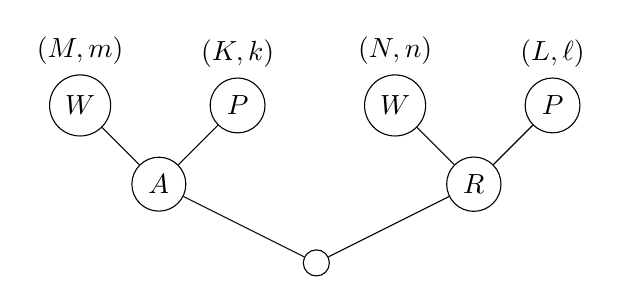
\begin{tikzpicture}
\path node (v0) at (0,0) [circle,draw] {} 
node (v1) at (-2,1) [circle,draw] {$A$} 
node (v2) at (-3,2) [circle,draw,label=above:{$(M,m)$}] {$W$} 
node (v3) at (-1,2) [circle,draw,label=above:{$(K,k)$}] {$P$} 
node (v4) at (1,2) [circle,draw,label=above:{$(N,n)$}] {$W$} 
node (v5) at (3,2) [circle,draw,label=above:{$(L,\ell)$}] {$P$} 
node (v6) at (2,1) [circle,draw] {$R$};
\draw (v0) -- (v1) -- (v2);
\draw (v1) -- (v3);
\draw (v0) -- (v6) -- (v5);
\draw (v6) -- (v4);
\end{tikzpicture}
$$
\alert{Conditional strategies:}
What would we do, if they did $X$? And what, if they did $Y$? 
\end{frame}  

\begin{frame}{Second payoff matrix: conditional strategies}

\begin{itemize}
\item Apollonia's moves: accept ($A$) or reject ($R$).
\item Tysq's moves:
\begin{itemize}  
\item $\frac{W}{W}$ -- war regardless of Apollonia's move,
\item $\frac{P}{P}$ -- peace regardless of Apollonia's move,
\item $\frac{W}{P}$ -- war if Apollonia accepts, peace if Apollonia rejects,
\item $\frac{P}{W}$ -- peace if Apollonia accepts, war if Apollonia rejects.
\end{itemize}
\end{itemize}
Here is the new payoff matrix:
\begin{center}
\begin{tabular}{c|cccc}
  & $\frac{W}{W}$ & $\frac{P}{P}$ & $\frac{W}{P}$ & $\frac{P}{W}$ \\
\hline
$A$ & $(M,m)$     & $(K,k)$       & $(M,m)$       & $(K,k)$  \\
$R$ & $(N,n)$     & $(L,\ell)$    & $(L,\ell)$    & $(N,n)$  
\end{tabular}
\end{center}
Note that the payoff values do not change. We still have
$M<N<K<L$ and $m < k$, $\ell < n$.
\end{frame}

\begin{frame}{Best responses}

\begin{enumerate}
\item If T. plays $\frac{W}{W}$, A.'s best response is 
$R$, because $M<N$.
\item If T. plays $\frac{P}{P}$, A.'s best response is
$R$, because $K<L$.
\item If T. plays $\frac{W}{P}$, A.'s best response is 
$R$, because $M<L$.
\item If T. plays $\frac{P}{W}$, A.'s best response is
$A$, because $N<K$.
\end{enumerate}
Apollonia does not have a move that is always better. In technical terms: 
Apollonia does not have a \alert{dominant} strategy. 

\begin{enumerate}
\item If A. plays $A$, T.'s best response is either 
$\frac{P}{P}$ or $\frac{P}{W}$, as $k>m$.
\item If A. plays $R$, T.'s best response is either 
$\frac{W}{W}$ or $\frac{P}{W}$, as $n>\ell$.
\end{enumerate}
Tysq does not have a dominant strategy. But Tysq has
a \alert{strictly dominated} strategy: a strategy that is never a best response
to anything, namely, $\frac{W}{P}$. Such a strategy should never be played by a
rational player!

\end{frame}

\begin{frame}{Third payoff matrix: Nash equilibria}

\begin{itemize}
\item Apollonia's moves: accept ($A$) or reject ($R$).
\item Tysq's moves:
\begin{itemize}  
\item $\frac{W}{W}$ -- war regardless of Apollonia's move,
\item $\frac{P}{P}$ -- peace regardless of Apollonia's move,
\item $\frac{P}{W}$ -- peace if Apollonia accepts, war if Apollonia rejects.
\end{itemize}
\end{itemize}
Here is the payoff matrix:
\begin{center}
\begin{tabular}{c|ccc}
  & $\frac{W}{W}$  & $\frac{P}{P}$  & $\frac{P}{W}$ \\
\hline
$A$ & $(M,m)$      & $(K,k)$        & $(K,k)^\star$  \\
$R$ & $(N,n)^\star$ & $(L,\ell)$     & $(N,n)$  
\end{tabular}
\end{center}

\begin{block}{Nash equilibria:}
The starred outcomes are such that no player has a strict incentive to move away
from one, if the other player is kept fixed.
\end{block}  

\end{frame}

\begin{frame}{Fourth payoff matrix and expected utilities}
The column $\frac{P}{P}$ is unstable: either one or the other player will have a
strict incentive to move away from it. The strategy $\frac{P}{P}$ should not be
played by a rational player! So, the final payoff matrix is:
\begin{center}
\begin{tabular}{c|cc}
  & $\frac{W}{W}$    & $\frac{P}{W}$ \\
\hline
$A$ & $(M,m)$        & $(K,k)^\star$  \\
$R$ & $(N,n)^\star$   & $(N,n)$  
\end{tabular}
\end{center}

\begin{itemize}
\item Decide on a strategy by calculating its \alert{expected utility}.
\end{itemize}

Let $p$ be the probability of Tysq playing $\frac{W}{W}$. Then, the probability
of Tysq playing $\frac{P}{W}$ is $1-p$.

\begin{block}{Apollonia's expected utilities:}
\begin{itemize}
\item $EU_A = pM +(1-p)K$  (e.u. of playing $A$)
\item $EU_R = pN +(1-p)N = N$ (e.u. of playing $R$)
\end{itemize}  
\end{block}

\end{frame}  

\section{Choice of strategy}
\subsection{}

\begin{frame}{How to choose a strategy}

The strategy Apollonia should choose, according to game-theoretic wisdom (and
common sense), is to
\begin{itemize}
\item play $A$ if $EU_A > EU_R$,
\item play $R$ if $EU_A < EU_R$,
\item play a randomised mix of $A$ and $R$ if $EU_A = EU_R$.
\end{itemize}

Recall that $M<N<K<L$. Let
\begin{itemize}
\item $S = K-M$ (the value of peace),
\item $H = N-M$ (the price of honour).
\end{itemize}
Now $S>H$, so $0<\frac{H}{S} <1$. By simple calculations, we obtain:
\begin{itemize}
\item play $A$ if $\frac{H}{S} < 1-p$,
\item play $R$ if $\frac{H}{S} > 1-p$,
\item play mix if $\frac{H}{S} = 1-p$.
\end{itemize}

\end{frame}    

\begin{frame}{Oracle's questions}

\begin{itemize}  
\item The first question is about $p$. This can be quite direct.
\item The second question is about $\frac{H}{S}$. How big is $H$ in comparison
  to $S$? This must be 
asked in a roundabout way if the oracle does not want to
give an introductory lecture on game theory. 
\end{itemize}

\begin{block}{What really happened on Xemya?}
\pause
I know, because I am from Xemya myself. You probably have guessed that. You are
also not mistaken if you think I am from Apollonia. But the real story is not
for today. 
\end{block}

\vfill
\pause
{\Huge Thank you!}

\end{frame}  


\end{document}

%%% Local Variables:
%%% mode: latex
%%% TeX-master: t
%%% End:


calculated as before but with payoffs from the row $R$. The strategy Apollonia
should choose, according to game-theoretic wisdom, is 
\begin{itemize}
\item $A$ if $EU_A > EU_R$,
\item $R$ if $EU_A < EU_R$,
\item a randomised mix of $A$ and $R$ if $EU_A = EU_R$.
\end{itemize}
